% ****** Start of file aipsamp.tex ******
%
%   This file is part of the AIP files in the AIP distribution for REVTeX 4.
%   Version 4.1 of REVTeX, October 2009
%
%   Copyright (c) 2009 American Institute of Physics.
%
%   See the AIP README file for restrictions and more information.
%
% TeX'ing this file requires that you have AMS-LaTeX 2.0 installed
% as well as the rest of the prerequisites for REVTeX 4.1
%
% It also requires running BibTeX. The commands are as follows:
%
%  1)  latex  aipsamp
%  2)  bibtex aipsamp
%  3)  latex  aipsamp
%  4)  latex  aipsamp
%
% Use this file as a source of example code for your aip document.
% Use the file aiptemplate.tex as a template for your document.
\documentclass[%
notitlepage,
 %reprint,%
%author-year,%
%author-numerical,%
%draft,
]{revtex4-1}

\usepackage{graphicx}% Include figure files
\usepackage{dcolumn}% Align table columns on decimal point
\usepackage{bm}% bold math

% packages added by Anand
\usepackage{subfig}
\usepackage{color}
\usepackage{amsmath}
\usepackage{amssymb}
\usepackage{xspace}
\usepackage{multirow}
\usepackage{bm}
%\usepackage[mathlines]{lineno}% Enable numbering of text and display math
%\linenumbers\relax % Commence numbering lines
\include{custom_commands}
\everymath{\displaystyle}

\newcommand{\pd}[2]{\frac{\partial #1}{\partial #2}}
\newcommand{\be}{\ensuremath{{\beta}}\xspace}
\newcommand{\ret}{\ensuremath{ Re_{\theta} \xspace}}
\renewcommand{\bm}{\ensuremath{{\boldsymbol\beta_{MAP}}}\xspace}
\newcommand{\mat}[1]{{\ensuremath{\bf{ #1}}}}
% comment the following lines to see figures
%\usepackage{ifdraft}
%\ifdraft{\renewcommand{\includegraphics}{\relax}}{\relax}
%\renewcommand{\includegraphics}[2][]{}
%\renewcommand{\subfloat}[0]{}
\usepackage{url}

\begin{document}

\preprint{}

\title[]{One Dimensional Channel,  Stress -- $\omega$ model }% Force line breaks with \\
%\thanks{Footnote to title of article.}

\author{Anand Pratap Singh}
\email{anandps@umich.edu}
\affiliation{Department of Aerospace Engineering, University of Michigan, Ann Arbor, MI 48109, USA}%

\date{\today}% It is always \today, today,
             %  but any date may be explicitly specified

\begin{abstract}

\end{abstract}

%\pacs{Valid PACS appear here}% PACS, the Physics and Astronomy
                             % Classification Scheme.
%\keywords{Suggested keywords}%Use showkeys class option if keyword
                              %display desired
\maketitle
\tableofcontents
\vspace{1cm}
\texttt{code: https://github.com/anandpratap/pyreystress (private repository)}
\section{Introduction}
\section{Stress - $\omega$}
\begin{figure}[!h]		
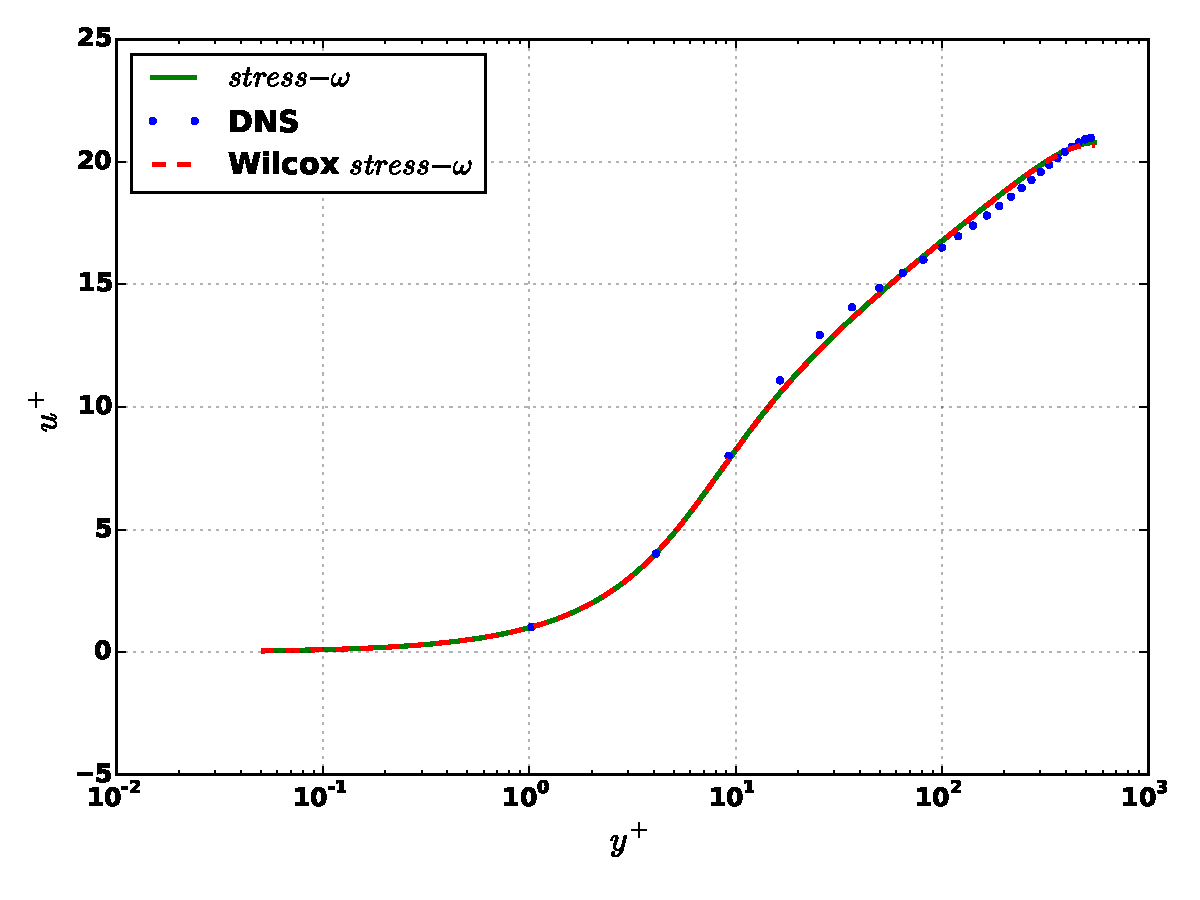
\includegraphics[width=0.8\linewidth]{figs/stress_omega/Re550/stress_omega_u.pdf}
\end{figure}
\begin{figure}[!h]		
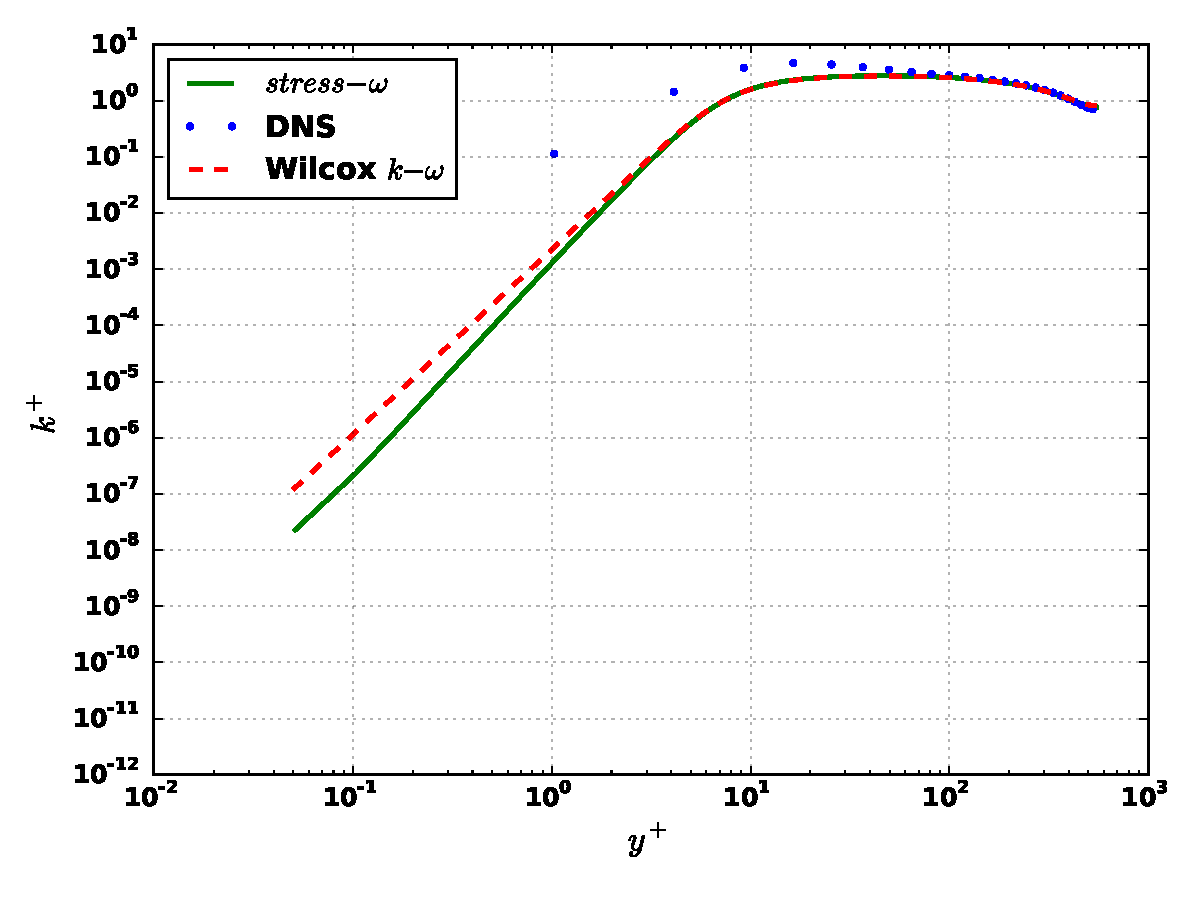
\includegraphics[width=0.8\linewidth]{figs/stress_omega/Re550/stress_omega_k.pdf}
\end{figure}
\begin{figure}[!h]		
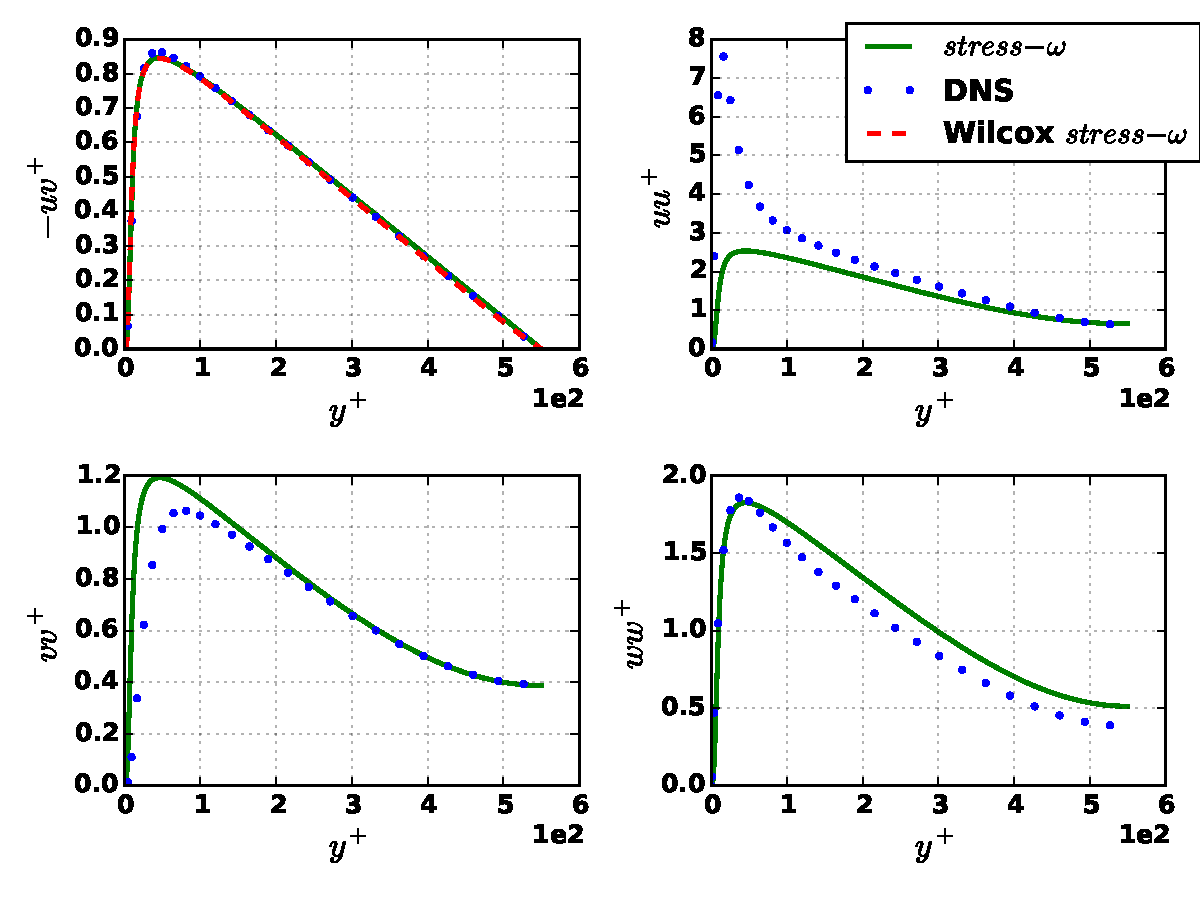
\includegraphics[width=0.8\linewidth]{figs/stress_omega/Re550/stress_omega_reystress.pdf}
\end{figure}
\appendix
\section{Stress--$\omega$ model}
\begin{eqnarray}
  \pd{}{y}\left(\nu \pd{u}{y} + R_{12}\right) - dp = 0\\
\end{eqnarray}
\begin{eqnarray}
  -P_{11} + \hat{\epsilon} + \epsilon_{11} - \Pi_{11} + \pd{}{y}\left[\left(\nu + \sigma^{\star} \nu_t\right)\pd{R_{11}}{y}\right] = 0\\ 
  -P_{12} + \epsilon_{12} - \Pi_{12} + \pd{}{y}\left[\left(\nu + \sigma^{\star} \nu_t\right)\pd{R_{12}}{y}\right] = 0 \\
 -P_{22} + \hat{\epsilon} + \epsilon_{22} - \Pi_{22} + \pd{}{y}\left[\left(\nu + \sigma^{\star} \nu_t\right)\pd{R_{22}}{y}\right] = 0\\
 -P_{33} + \hat{\epsilon} + \epsilon_{33} - \Pi_{33} + \pd{}{y}\left[\left(\nu + \sigma^{\star} \nu_t\right)\pd{R_{33}}{y}\right] = 0 
\end{eqnarray}
\begin{eqnarray}
  P_{11} = 2 R_{12}\pd{u}{y}\\ 
  P_{12} = R_{22}\pd{u}{y}\\ 
  P_{22} = 0\\
  P_{33} = 0
\end{eqnarray}

\begin{eqnarray}
  D_{11} = 0\\
  D_{12} = R_{11}\pd{u}{y}\\ 
  D_{22} = 2 R_{12}\pd{u}{y}\\ 
  D_{33} = 0
\end{eqnarray}

\begin{eqnarray}
  S_{11} = 0\\
  S_{12} = \frac{1}{2}\pd{u}{y}\\
  S_{22} = 0\\
  S_{33} = 0
\end{eqnarray}
\begin{eqnarray}
  \Pi_{11} = \beta^{\star}C_1\omega\left(R_{11} + \frac{2}{3}k\right) - \hat{\alpha}\left(P_{11} - \frac{2}{3}P_{trace}\right) - \hat{\beta}\left(D_{11} - \frac{2}{3}P_{trace}\right) - \hat{\gamma}\left(S_{11} - \frac{1}{3}S_{trace}\right)\\
  \Pi_{12} = \beta^{\star}C_1\omega R_{12} - \hat{\alpha} P_{12} - \hat{\beta} D_{12}- \hat{\gamma} S_{12}\\
  \Pi_{22} = \beta^{\star}C_1\omega\left(R_{22} + \frac{2}{3}k\right) - \hat{\alpha}\left(P_{22} - \frac{2}{3}P_{trace}\right) - \hat{\beta}\left(D_{22} - \frac{2}{3}P_{trace}\right) - \hat{\gamma}\left(S_{22} - \frac{1}{3}S_{trace}\right)\\
  \Pi_{33} = \beta^{\star}C_1\omega\left(R_{33} + \frac{2}{3}k\right) - \hat{\alpha}\left(P_{33} - \frac{2}{3}P_{trace}\right) - \hat{\beta}\left(D_{33} - \frac{2}{3}P_{trace}\right) - \hat{\gamma}\left(S_{33} - \frac{1}{3}S_{trace}\right)\\
\end{eqnarray}


\begin{eqnarray}
  \hat{\epsilon} = \frac{2}{3}\beta^{\star}k \omega\\
  \epsilon_{11} = -\frac{1}{4}\nu \pd{^{2}R_{11}}{y^2}\\ 
  \epsilon_{12} = -\frac{1}{4}\nu \pd{^{2}R_{12}}{y^2}\\ 
  \epsilon_{22} = -\frac{1}{4}\nu \pd{^{2}R_{22}}{y^2}\\ 
  \epsilon_{33} = -\frac{1}{4}\nu \pd{^{2}R_{33}}{y^2}\\ 
\end{eqnarray}
\begin{eqnarray}
  P_{trace} = \frac{1}{2}(P_{11} + P_{22} + P_{33})\\
  S_{trace} = S_{11} + S_{22} + S_{33}\\
  k = -\frac{1}{2}\left(R_{11} + R_{22} + R_{33}\right)\\
  \nu_t = \frac{k}{\omega}
\end{eqnarray}
\begin{eqnarray}
\frac{\alpha \omega R_{12}}{k}\pd{u}{y} - \beta_{0}\omega^2 +\pd{}{y}\left[\left(\nu - \sigma\nu_t\right)\pd{\omega}{y}\right] + \max\left(\frac{1}{8\omega}\pd{k}{y}\pd{\omega}{y}, 0\right) = 0 \\
\end{eqnarray}

\begin{eqnarray}
    C_1 = \frac{9}{5}\\
    C_2 = \frac{10}{19}\\
    \alpha_h = \frac{8 + C2}{11}\\
    \alpha = \frac{13}{25}\\
    \sigma = 0.5\\
    \beta_0 = 0.0708\\
    \beta_\star = \frac{9}{100}\\
    \sigma_\star = 0.6\\
    \sigma_{do} = \frac{1}{8}\\
    \hat{\alpha} = \frac{8 + C_2}{11}\\
    \hat{\beta} = \frac{8C_2 - 2}{11}\\
    \hat{\gamma} = \frac{60C_2 - 4}{55}\\
\end{eqnarray}

\end{document}

%
% ****** End of file aipsamp.tex ******
